\documentclass{beamer}


\mode<presentation>
{
  \usetheme{Darmstadt}
  \useoutertheme{infolines}
}

\usepackage{alltt}

\usepackage{etex}         % to avoid compilation erros of xypic
\usepackage[curve]{xypic}
%\xyoption{pdf}
%\usepackage[pdf]{xy}


\usepackage[utf8]{inputenc}
\usepackage{proof}
\inferLineSkip=4pt  % increase spacing between lines; default is 2pt

\usepackage{amsmath}
\usepackage{amssymb}
\usepackage{fontawesome}
\usepackage{times}
\usepackage[T1]{fontenc}
\usepackage{listings}
\lstset{language=haskell,basicstyle=\ttfamily}

\usepackage{multicol}
\usepackage{mathpartir}
\usepackage{mathtools}
\usepackage{stmaryrd}
\usepackage{soul}
\usepackage{tikzsymbols}

% Delete this, if you do not want the table of contents to pop up at
% the beginning of each subsection:
\AtBeginSection[]
{
  \begin{frame}<beamer>
    \frametitle{Plan}
    \tableofcontents[sectionstyle=show/shaded,subsectionstyle=hide]
  \end{frame}
}

\AtBeginSubsection[]
{
  \begin{frame}<beamer>
    \frametitle{Plan}
    \tableofcontents[sectionstyle=show/hide,subsectionstyle=show/shaded/hide]
%    \tableofcontents[subsectionstyle=show/shaded/hide]
  \end{frame}
}

\setbeamertemplate{footline}
{%
%\begin{beamercolorbox}{section in head/foot}
%\vskip2pt\insertnavigation{\paperwidth}\vskip2pt
%\end{beamercolorbox}%
\insertpagenumber
\insertshorttitle[width={5cm},center]
\insertshortinstitute[width={3cm},center]
\insertshortdate[width={3cm},center]
}


% If you wish to uncover everything in a step-wise fashion, uncomment
% the following command: 

%\beamerdefaultoverlayspecification{<+->}

\usepackage{tikz}
\usetikzlibrary{trees}
\usetikzlibrary{arrows}
\usetikzlibrary{decorations.pathmorphing}
\usetikzlibrary{shapes.multipart}
\usetikzlibrary{shapes.geometric}
\usetikzlibrary{calc}
\usetikzlibrary{positioning} 
\usetikzlibrary{fit}
\usetikzlibrary{backgrounds}
\usetikzlibrary{automata}


%%% Local Variables: 
%%% mode: latex
%%% TeX-master: "main"
%%% End: 

% Theorems and definitions

% \newtheorem{definition}{Definition}
% \newtheorem{theorem}{Theorem}
% \newtheorem{lemma}{Lemma}
% \newtheorem{proposition}{Proposition}


% Definition of colors
\newcommand{\blue}[1]{{\color{blue}#1}}
\newcommand{\green}[1]{{\color{green}#1}}
\newcommand{\red}[1]{{\color{red}#1}}
\newcommand{\gray}[1]{{\color{gray}#1}}

% From MSCS file
\newcommand{\eg}{\textit{e.g.\ }}
\newcommand{\etal}{\textit{et al.\ }}
\newcommand{\etc}{\textit{etc}}
\newcommand{\ie}{\textit{i.e.\ }}
\newcommand{\viz}{\textit{viz.\ }}
\newcommand{\wrt}{\textit{w.r.t.\ }}
\newcommand{\lex}{\langle}
\newcommand{\rex}{\rangle}

% Own abbreviations
\newcommand{\secref}[1]{Section~\ref{#1}}
\newcommand{\secrefs}[1]{Sections~\ref{#1}}
\newcommand{\figref}[1]{Figure~\ref{#1}}
\newcommand{\figrefs}[1]{Figures~\ref{#1}}
\newcommand{\pgref}[1]{page~\pageref{#1}}
\newcommand{\theoremref}[1]{Theorem~\ref{#1}}
\newcommand{\theoremrefs}[1]{Theorems~\ref{#1}}
\newcommand{\lemmaref}[1]{Lemma~\ref{#1}}
\newcommand{\exampleref}[1]{Example~\ref{#1}}
\newcommand{\defref}[1]{Definition~\ref{#1}}

\newcommand{\figline}{\rule{\textwidth}{0.5pt}}


% Logique

\newcommand{\IMPL}[0]{\longrightarrow}
\newcommand{\IMPLL}[0]{\Longrightarrow} % another implication, to make
                                % a difference with reduction relations
\newcommand{\AND}[0]{\land}
\newcommand{\OR}[0]{\lor}
\newcommand{\NOT}[0]{\lnot}
\newcommand{\FALSE}[0]{\perp}
\newcommand{\TRUE}[0]{\top}
\newcommand{\IFF}[0]{\leftrightarrow}
\newcommand{\BIGAND}[1]{\bigwedge_{#1}}
\newcommand{\BIGOR}[1]{\bigvee_{#1}}
\newcommand{\BIGANDC}[2]{\bigwedge_{#1|#2}} % bigand with constraint
\newcommand{\BIGORC}[2]{\bigvee_{#1|#2}}    % bigor with constraint

\newcommand{\exgeq}[1]{\exists^{{\geq #1}}}
\newcommand{\exeq}[1]{\exists^{{= #1}}}
\newcommand{\exle}[1]{\exists^{{< #1}}}

% Other

\newcommand{\smalltalcq}[0]{{\small small}-t{$\cal ALCQ$}}
\newcommand{\smalltalcqe}[0]{{\small small}-t{$\cal ALCQ$e}}
\newcommand{\trule}[0]{\xhookrightarrow}
\newcommand{\tableaurule}[1]{{\xhookrightarrow[]{#1}}}
\newcommand{\nodes}[1]{{\cal N}({#1})}
\newcommand{\trans}[1]{{\cal T}({#1})}
\newcommand{\transm}[1]{{\cal T'}({#1})}
\newcommand{\rconts}[1]{\llparenthesis #1 \rrparenthesis} %record contents
\newcommand{\rupd}[2]{{#1}\llparenthesis #2 \rrparenthesis} %record update

\newcommand{\eform}[0]{\mathit{eform}}
\newcommand{\form}[0]{\mathit{form}}
\newcommand{\free}[0]{\mathit{free}}
\newcommand{\exclprop}[0]{\stackrel{\times}{\longrightarrow}}


%----------------------------------------------------------------------
% For drawing syntax diagrams
% ----------------------------------------------------------------------

% Environment defining the general layout

\newenvironment{syntaxdiagram}[1]
{
%  \begin{equation}\label{eq:#1}
  \begin{tikzpicture}[%
node distance=5mm and 10mm,
>=stealth',
black!50,
text=black,
graphs/every graph/.style={edges=rounded corners},
hv path/.style={to path={-| (\tikztotarget)}},
vh path/.style={to path={|- (\tikztotarget)}},
nonterminal/.style={%
rectangle,
minimum size=6mm,
draw=black,
},
terminal/.style={%
rectangle,minimum size=6mm,rounded corners=3mm,
draw=black!50,
},
start/.style={%
circle,inner sep=1pt,minimum size=1pt,fill=white,draw=black!50,
},
end/.style={%
start,
},
junction/.style={circle,inner sep=0pt,minimum size=0pt},]
\node[nonterminal] (#1) {\hypertarget{syn:#1}{#1:}};
}
{\end{tikzpicture}
%\end{equation}
}

% Connects start point #1 via intermediate node entry #2 and exit #3
% to an end point #4.
\newcommand{\syndiagAlternative}[4]{%
\graph[use existing nodes] {
#1 ->[vh path] #2;
#3 ->[hv path] #4;
};
}

% Connects start point #1 via intermediate node #2 (typically a junction)
% to an end point #3.
\newcommand{\syndiagBridge}[3]{%
\graph[use existing nodes] {
#1 --[vh path] #2;
#2 ->[hv path] #3;
};
}

\newcommand{\nonterminalref}[1]{\hyperlink{syn:#1}{#1}}


%----------------------------------------------------------------------
% Remarks
% ----------------------------------------------------------------------

\newcommand{\remms}[2][]{\todo[color=green!40,#1]{MS: #2}}



%%% Local Variables: 
%%% mode: latex
%%% TeX-master: "main"
%%% End: 


\title{L4 design}

\author{Martin Strecker}
\date{2021-03-02}


%======================================================================

\begin{document}


%======================================================================

\begin{frame}
  \titlepage
\end{frame}



%======================================================================
\section{Snapshot: Baby-L4 now}

%-------------------------------------------------------------
\begin{frame}[fragile]\frametitle{General structure of an L4 file}

  \begin{itemize}
  \item Lexicon
\begin{alltt}
\textbf{lexicon}
Business -> business_2 #from WordNet
Value -> value_1 
\end{alltt}
    
  \item List of class definitions (class $\approx$ type):
\begin{alltt}
\textbf{class} Business \{
      foo: Int
      bar: Bool -> (Int,Int)
\}

\textbf{class} LawRelatedService \textbf{extends} Business \{
\}
\end{alltt}

    
  \end{itemize}

\end{frame}


%-------------------------------------------------------------
\begin{frame}[fragile]\frametitle{General structure of an L4 file}

  \begin{itemize}
  \item Declarations:
\begin{alltt}
\textbf{decl} AssociatedWith: LegalPractitioner -> 
                      Appointment -> Bool
\textbf{decl} MayAcceptApp : LegalPractitioner -> 
                      Appointment -> Bool
\textbf{decl} ProhibitedBusiness : Business -> Bool
\end{alltt}
    
  \end{itemize}

\end{frame}

%-------------------------------------------------------------
\begin{frame}[fragile]\frametitle{General structure of an L4 file}


  \begin{itemize}
  \item Rules:
\begin{alltt}
\textbf{rule} <r1a>
\textbf{for} lpr: LegalPractitioner, app: Appointment
\textbf{if} (exists bsn : Business. 
         AssociatedWithAppB app bsn 
      \&\& IncompatibleDignity bsn)
\textbf{then} MustNotAcceptApp lpr app
\end{alltt}
  
\item Assertions / Goals to be proved:
\begin{alltt}
\textbf{assert} 
  exists lpr: LegalPractitioner. 
  exists app: Appointment. 
      MayAcceptApp lpr app
\end{alltt}
  \end{itemize}

\end{frame}

  
%======================================================================
\section{What to do with Baby-L4}

%-------------------------------------------------------------
\subsection{The space of options}
%-------------------------------------------------------------


%-------------------------------------------------------------
\begin{frame}[fragile]\frametitle{Class definitions}

  \blue{Purpose:}
  \begin{itemize}
  \item Separation of data and ``rules''
  \item Used in type checking
  \end{itemize}
  
  \blue{What to do with it?}
  \begin{itemize}
  \item Parse data from data description languages:\\
    YAML, Jason, \dots\\
    \dots and check conformity with class defs
  \item Generate language stubs for OO languages
  \item Use in verification tools like Alloy
  \end{itemize}

\end{frame}

%-------------------------------------------------------------
\begin{frame}[fragile]\frametitle{Semantics of classes and fields}

  \blue{Mathematically:} Class = set of objects

  \blue{Pragmatically:}
  \begin{itemize}
  \item Fields corrsponding to relation declarations?
  \item Fields/ methods in the sense of OO languages?
  \end{itemize}
  Complementary, not incompatible views.

\end{frame}


%-------------------------------------------------------------
\begin{frame}[fragile]\frametitle{Semantics of classes and fields}

  \blue{Fields as function / relation declarations?}

\begin{alltt}
\textbf{class} LegalPractitioner \textbf{extends} Person \{
\}
\textbf{decl} AssociatedWith:
     LegalPractitioner -> Appointment -> Bool
\end{alltt}
  
the same as?:

\begin{alltt}
\textbf{class} LegalPractitioner \textbf{extends} Person \{
    AssociatedWith: Appointment -> Bool
\}
\end{alltt}

Functional / relational view: we write

\begin{alltt}
  forall lpr  : LegalPractitioner.
  exists app: Appointment.
     AssociatedWith lpr app
\end{alltt}

\end{frame}


%-------------------------------------------------------------
\begin{frame}[fragile]\frametitle{Semantics of classes and fields}

  \blue{Fields as components of a record}


  ``Relational'' view of components (as in Alloy)
\begin{alltt}
\textbf{class} LegalPractitioner \textbf{extends} Person \{
    salary: Int
\}
\end{alltt}

Understanding: \texttt{salary} is a relation\\
\texttt{LegalPractitioner} $\times$ \texttt{Int}

and \texttt{lpr.salary} is relation composition.

\end{frame}

%-------------------------------------------------------------
\begin{frame}[fragile]\frametitle{Semantics of classes and fields}

  \blue{Fields as components of a record}


  ``Functional'' view of components:
\begin{alltt}
\textbf{class} LegalPractitioner \textbf{extends} Person \{
      salary: Int
\}
\end{alltt}

For \texttt{lpr: LegalPractitioner}, one can write:\\
\texttt{lpr.salary}

which is syntactic sugar of \texttt{salary(lpr)}

\red{Downside:} under the relational interpretation, \texttt{lpr.salary} is
not uniquely determined $\leadsto$ cardinality annotations.

\end{frame}
  
%-------------------------------------------------------------
\subsection{Proposal}
%-------------------------------------------------------------

%-------------------------------------------------------------
\begin{frame}[fragile]\frametitle{Core / operational / logical model}

  \blue{Core model} describes the essential semantics of constructs

  \vspace{5mm}
  \blue{Operational model} for use in programming languages

  \vspace{5mm}
  \blue{Logical model} for use in verification tools.

\end{frame}


%-------------------------------------------------------------
\begin{frame}[fragile]\frametitle{Core model: Types}

  The elements of discourse are characterized by
  \blue{types}
  \begin{itemize}
  \item \emph{Predefined} types (\texttt{int}, \texttt{bool}) represent sets of
    numbers / truth values
  \item \emph{Classes} are specific types representing \emph{objects}
  \item So far no inductively defined \texttt{data} types
  \end{itemize}

  \vspace{5mm}
  Syntactic restrictions imposed on \blue{classes}:
  \begin{itemize}
  \item Classes arranged in hierarchy (\texttt{extends})
    \begin{itemize}
    \item that must be acyclic
    \item with top class \texttt{Object}
    \end{itemize}
  \item Unique field names (no overriding)
  \end{itemize}

\end{frame}


%-------------------------------------------------------------
\begin{frame}[fragile]\frametitle{Core model: Instances}

  Instances and the question of identity:   Given a class
\begin{alltt}
\textbf{class} Person \{
      name: String
      spouse: Person
\}
\end{alltt}
how to marry \texttt{jane} and \texttt{jim}?
\begin{alltt}
  \textbf{def} jane =
       \{ name = "Jane",
         spouse = \{ name = "Jim",
                    spouse = \{ name = "Jane", ...
\end{alltt}
Not practicable.

\end{frame}

%-------------------------------------------------------------
\begin{frame}[fragile]\frametitle{Core model: Instances}

  Reference-based model:
\begin{alltt}
\textbf{decl} jane: Person
\textbf{decl} jim: Person
\textbf{def} jane = \textbf{instance} Person
       \{ name = "Jane",
         spouse = jim \}
\textbf{def} jim = \textbf{instance} Person
       \{ name = "Jim",
         spouse = jane \}
\end{alltt}

Here: \textbf{\texttt{instance}} creates an object identity:

\begin{alltt}
\textbf{class} Object \{
   id: Integer
\}
\end{alltt}

\end{frame}

%-------------------------------------------------------------
\begin{frame}[fragile]\frametitle{Core model: Instances}

  Unpleasant: object identities not directly visible:

  \begin{alltt}
\textbf{def} oedipusJr = \textbf{instance} Person
                \{name = "Oedipus",
                 spouse = jocasta
\}
\textbf{def} oedipusSen = \textbf{instance} Person
                 \{name = "Oedipus",
                  spouse = jocasta
\}
  \end{alltt}    

  with \texttt{oedipusJr} $\neq$ \texttt{oedipusSen}
  
\end{frame}

%-------------------------------------------------------------
\begin{frame}[fragile]\frametitle{Core model: Instances}

  Semantics? Classical heap-based semantics with state:

  \begin{itemize}
  \item $state = heap \times locals$
  \item $locals = VarName \to val$
  \item $heap = objid \to obj$
  \item $obj = ClassName \times [FieldName \to val]$
  \end{itemize}

  The heap remains constant after reading all \textbf{def}s.

  Or doesn't it?

\end{frame}


%-------------------------------------------------------------
\begin{frame}[fragile]\frametitle{Core model: Dynamics}

  \blue{Functions in classes?}
\begin{alltt}
\textbf{class} Tax \{
      taxCalc: Int -> Int
\}
\end{alltt}

Not a good idea: \texttt{t1, t2: Tax} could not be compared.

\end{frame}


%-------------------------------------------------------------
\begin{frame}[fragile]\frametitle{Operational model}

\end{frame}



%======================================================================
\section{Moving to L4}


%-------------------------------------------------------------
\begin{frame}[fragile]\frametitle{Rule modifiers}

  ... such as \texttt{subject to} clauses:

  \begin{itemize}
  \item annotations in rules 
  \item compilation of preconditions
  \end{itemize}


\end{frame}


%-------------------------------------------------------------
\begin{frame}[fragile]\frametitle{Deontic statements}

  Further investigations:

  \begin{itemize}
  \item Obligations as requirements on a module
  \item Permissions as requirements on its environment
  \item Composition of contracts
  \item Rely-Guarantee reaasoning
  \end{itemize}

\end{frame}


%======================================================================
\section{Contracts}


%-------------------------------------------------------------
\begin{frame}[fragile]\frametitle{Review of related approaches}

  \begin{itemize}
  \item FCL, by Quian Hu / William Farmer
  \item CSL, by Deon Digital
  \end{itemize}

\end{frame}

% -------------------------------------------------------------
\subsection{FCL}
% -------------------------------------------------------------

%-------------------------------------------------------------
\begin{frame}[fragile]\frametitle{FCL}

  FCL
  \begin{itemize}
  \item PhD thesis of Quian Hu
  \item supervised by William Farmer (``Little Theories'')
  \end{itemize}

  \vspace{5mm}
  General appreciation:
  \begin{itemize}
  \item In PhD thesis: Lengthy explication of some fundamentals (``simple type
    theory'')
  \item Few references to established notions (automata / temporal logics)
  \item Not clear whether there exists a real implementation 
  \item One minimalistic example in the appendix
  \end{itemize}


\end{frame}

%-------------------------------------------------------------
\begin{frame}[fragile]\frametitle{FCL: Notion of contract}



  \begin{itemize}
  \item Contract $C = (t, Q)$ where:
    \begin{itemize}
    \item $t$ is the ``current'' time
    \item $Q$ is a set of constant definitions $D$, agreements $A$, rules $R$
    \end{itemize}
    
  \item Rule $R$ is of the form $\phi \mapsto Q$, where $\phi$ is a formula\\
    ``if $\phi$ is satisfied at time $t$, the elements of $Q$ are added to the
    state at $t+1$''

  \item Agreement $A$ is of the form $O(a, T)$ or $F(a, T)$ where
    \begin{itemize}
    \item $a$ is an action
    \item $T$ a set of times
    \item $O$ expresses an obligation and $F$ a prohibition (forbidden)
    \end{itemize}
  \end{itemize}

\end{frame}

%-------------------------------------------------------------
\begin{frame}[fragile]\frametitle{FCL: Semantics}


  Obligations / prohibitions:
  \begin{itemize}
  \item   Obligation $O(a, T)$ corresponds to\\
    $\exists u : Time. u \in T \AND u \leq t \AND \mathit{obs-event}(u,a)$
  \item  $F(a, T) = \NOT O(a, T)$
  \end{itemize}
  
  Contracts:
  \begin{itemize}
  \item Evolving in discrete time steps
  \item New rules $\phi \mapsto Q$ are ``activated'' when their precondition
    $\phi$ becomes active
  \end{itemize}


\end{frame}

%-------------------------------------------------------------
\begin{frame}[fragile]\frametitle{Remarks about FCL}

  \begin{itemize}
  \item Permissions as obligations imposed on others
  \item However: Obligations / prohibitions not bound to a principal 
  \item Contracts no first-order entities (no operators on contracts)
  \item In particular, no composition of contracts
  \end{itemize}

\end{frame}

% -------------------------------------------------------------
\subsection{CSL}
% -------------------------------------------------------------

%-------------------------------------------------------------
\begin{frame}[fragile]\frametitle{Background: Process Algebras}

  Purpose:
  \begin{itemize}
  \item provide an algebraic account of \emph{concurrent} systems
  \item  (whereas lambda calculus / combinatory algebra are for
    single-process, deterministic systems)
  \item defines a set of \emph{traces} that are valid executions of the system
  \end{itemize}

  Best known representatives (starting in the 1970):
  \begin{itemize}
  \item CCS (Calculus of Communicating Systems) by Robin Milner
  \item CSP (Communicating Sequential Processes) by CAR Hoare
  \end{itemize}

  Verification tools directly based on process algebras:
  \begin{itemize}
  \item LOTOS
  \item CADP \url{http://cadp.inria.fr/}
  \end{itemize}

\end{frame}

%-------------------------------------------------------------
\begin{frame}[fragile]\frametitle{CCS}

  Processes $p,q$ are built up of constructors:

  \begin{itemize}
  \item nil: empty process, stops immediately
  \item $a.p$: carry out action $a$, then behave like $p$
  \item $p + q$: nondeterministically behave like $p$ or $q$
  \item $p | q$: parallel composition of $p$ and $q$ (maybe synchronizing on
    an internal action)
  \item $rec\; x. p$: recursive process running $p$ and then restarting $rec\;
    x. p$
    
  \item Operators for hiding ($p \backslash a$) and renaming
  \end{itemize}

  Example derivations:
  \begin{itemize}
  \item $r := rec\; x. (a.b.x + a.c.x) \longrightarrow a.b.r + a.c.r
    \longrightarrow a.b.r \stackrel{a}{\longrightarrow}$\\
    $b.r \stackrel{b}{\longrightarrow} r \longrightarrow a.b.r + a.c.r
    \longrightarrow a.c.r \longrightarrow \dots$ 
  \item $(a.b.d | a.c.d)\backslash a \stackrel{\tau}{\longrightarrow} (b.d | c.d)\backslash a \stackrel{c}{\longrightarrow} 
    (b.d | d)\backslash a \longrightarrow \dots$ 
  \end{itemize}

\end{frame}

%-------------------------------------------------------------
\begin{frame}[fragile]\frametitle{CCS and automata}

  \begin{center}
$a . b . r + a . c . r \neq a. (b. r + c.r)$  
\end{center}

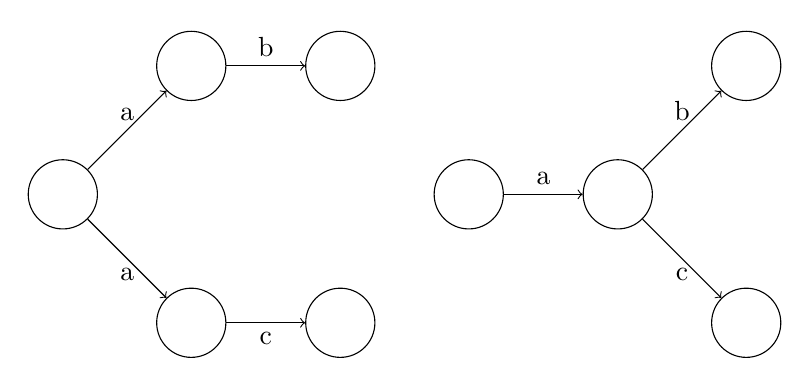
\begin{tikzpicture}[scale=.5]

  \node[state] (q0) {};
  \node[state] (qa1) [above right=of q0] {};
  \node[state] (qa2) [below right=of q0] {};
  \node[state] (qb) [right=of qa1] {};
  \node[state] (qc) [right=of qa2] {};

  \path[->] (q0) edge [above] node {a} (qa1)
                 edge [below] node {a} (qa2)
            (qa1) edge [above] node {b} (qb)
            (qa2) edge [below] node {c} (qc);

  \node[state] (q0') [below right=of qb] {};
  \node[state] (qa') [right=of q0'] {};
  \node[state] (qb') [above right=of qa'] {};
  \node[state] (qc') [below right=of qa'] {};

  \path[->] (q0') edge [above] node {a} (qa')
            (qa') edge [above] node {b} (qb')
            (qa') edge [below] node {c} (qc');

\end{tikzpicture}
\end{frame}

%-------------------------------------------------------------
\begin{frame}[fragile]\frametitle{CSL}

  CSL
  \begin{itemize}
  \item  Developed by Deon Digital
  \item based on PhD of Tom Hvitved, supervised by Henglein, Filinski
  \end{itemize}


  \vspace{5mm}
  General appreciation:
  \begin{itemize}
  \item PhD thesis discusses in fact two models:
    \begin{itemize}
    \item one based on Process Algebras
    \item one based on automata
    \end{itemize}
  \item \dots{} and lots of implementation details
  \item Concentrates on
    \begin{itemize}
    \item execution and run-time monitoring
    \item blame assignment (which party is responsible for breach)
    \item But: what about static verification?
    \end{itemize}
  \end{itemize}

  \red{Some notable differences between CSL-Deon and CSL by T.H.}
  
\end{frame}


%-------------------------------------------------------------
\begin{frame}[fragile]\frametitle{CSL - Deon}

  Essentially:
  \begin{itemize}
  \item a process algebra 
  \item without a specification mechanism for desired behavior (obligations / permissions)
  \end{itemize}

  Ingredients:
  \begin{itemize}
  \item ``final'' contracts: \texttt{success}, \texttt{failure}
  \item elementary contracts:\\
    \texttt{<AGENT> x:EVENTTYPE where PREDICATE}

    \emph{Example}
\begin{verbatim}
<buyer> order: BikeOrder where
      order.amount = 100 &&
      order.recipient = seller
\end{verbatim}
    
  \end{itemize}

\end{frame}


%-------------------------------------------------------------
\begin{frame}[fragile]\frametitle{CSL - Deon}

  Contract composition:
  \begin{itemize}
  \item Sequential: \texttt{c1 then c2}\\
    (more or less $c1 . c2$ in CCS)
  \item Nondeterministic choice: \texttt{c1 or c2}\\
    ($c1 + c2$ in CCS)
  \item Concurrent composition with interleaving: \texttt{c1 and c2}\\
    ($c1 | c2$ in CCS)
  \item Recursive congtracts \\
    \texttt{contract rec contractName = CONTRACTBODY}
  \end{itemize}

\end{frame}

%-------------------------------------------------------------
\begin{frame}[fragile]\frametitle{CSL - Deon}

\small
\begin{verbatim}
contract entrypoint sale3 = 
   \(buyer, seller, amount, item, inventory) ->
  // Some buyer orders an item for some price from a seller
  <buyer> order: Order where
      order.amount = amount &&
      order.recipient = seller &&
      order.item = item
  then (
    // The seller delivers that item
    <seller> delivery: Delivery where
        checkOffer inventory order.item order.amount &&  ...
  or
    // The seller tries to cheat
    <seller> delivery: Delivery where
        checkOffer inventory order.item order.amount && ...
    then failure
  )
\end{verbatim}
\normalsize


\end{frame}


%-------------------------------------------------------------
\begin{frame}[fragile]\frametitle{CSL - T.H.}

  Two major changes / additions:
  \begin{itemize}
  \item Atomic agent-initiated contracts replaced by obligations:\\
    \texttt{<agent> event(x1 ... xn) \textbf{where} cond \textbf{due} d \textbf{remaining} z \textbf{then} c}
  \item External choice:\\
    \texttt{\textbf{if} event(x1 ... xn)  \textbf{where} cond \textbf{due} d
      \textbf{remaining} z \textbf{then} c1 else \textbf{else} c2}
  \end{itemize}
  where \texttt{d} is a deadline: \texttt{\textbf{after} e2 \textbf{within} e2}


\end{frame}



%-------------------------------------------------------------
\begin{frame}[fragile]\frametitle{Interesting for L4}


\end{frame}



% -------------------------------------------------------------
\section{Automata}
% -------------------------------------------------------------

% -------------------------------------------------------------
\subsection{Introduction to Automata with JFLAP}
% -------------------------------------------------------------


%-------------------------------------------------------------
\begin{frame}[fragile]\frametitle{Downloading and starting JFLAP}


  Download site: \url{http://www.jflap.org/jflaptmp/}

  How to run it?
  \begin{itemize}
  \item Install Java 
  \item \texttt{java -jar JFLAP7.1.jar\&}
  \end{itemize}

  Tutorial: \url{http://www.jflap.org/tutorial/}

\end{frame}


%-------------------------------------------------------------
\begin{frame}[fragile]\frametitle{The trinity}

  \blue{Three essential notions:}
  \begin{itemize}
  \item \emph{Languages} as sets of strings made up of symbols.

    Examples: 

    \begin{itemize}
    \item The set of legal identifiers:
      $L_1 = \{ a, a\_1, b2, xyz, myVar, \dots \}$

      Note: $2b \notin L_1$
    \item The set of legal positive numbers:
      $L_2 = \{ 1, 11, 21, 42, 2021, \dots \}$

      Note: $007 \notin L_2$
    \end{itemize}

    
  \item \emph{Grammars} for a compact representation of languages
  \item \emph{Automata} for recognizing languages
  \end{itemize}

  \blue{Questions:}
  \begin{itemize}
  \item Can every language be represented by a grammar?
  \item What is the relation between grammars and automata?
  \end{itemize}

\end{frame}


%-------------------------------------------------------------
\begin{frame}[fragile]\frametitle{Automata in JFLAP}

  The chewing gum vending automaton

  \begin{onlyenv}<1>
    \blue{Scenario~1:}
    \begin{enumerate}
    \item Insert two dollars.
    \item Get chewing gum.
    \item Chew it.
    \end{enumerate}

    \blue{Actions:}

    \begin{itemize}
    \item $d$: insert one dollar
    \item $g$: get chewing gum
    \item $c$: chew for one hour
    \end{itemize}

    Corresponding \blue{language}: $ddgc$
  \end{onlyenv}

  \begin{onlyenv}<2>
    \blue{Scenario~2:}
    \begin{enumerate}
    \item Insert two dollars.
    \item Get chewing gum.
    \item If you travel to Singapore: chew for one hour, then go to prison
    \item If you travel to Europe: chew for one hour, then get toothache
    \end{enumerate}

    \blue{Actions:}

    \begin{itemize}
    \item $d$: insert one dollar
    \item $g$: get chewing gum
    \item $c$: chew for one hour
    \item $s$~/~$e$: travel to Singapore / Europe
    \item $p$: go to prison
    \item $a$: get toothache
    \end{itemize}

    Corresponding \blue{language}: $ddg(scp|eca)$
  \end{onlyenv}


  \begin{onlyenv}<3>
    \blue{Scenario~3:} as Scenario~2, but:
    \begin{itemize}
    \item If in Europe: chew until you get toothache
    \end{itemize}

    \blue{Actions:}

    \begin{itemize}
    \item $d$: insert one dollar
    \item $g$: get chewing gum
    \item $c$: chew for one hour
    \item $s$~/~$e$: travel to Singapore / Europe
    \item $p$: go to prison
    \item $a$: get toothache
    \end{itemize}

    Corresponding \blue{language}: $ddg(scp|e(c^*)a)$
  \end{onlyenv}


  
  \begin{onlyenv}<4>
    \blue{Scenario~4:} as Scenario~3, but:
    \begin{itemize}
    \item If in Singapore: be released from prison, start chewing again, go to prison again (indefinitely) until you throw away the chewing gum. 
    \end{itemize}

    \blue{Actions:}

    \begin{itemize}
    \item $d$: insert one dollar
    \item $g$: get chewing gum
    \item $c$: chew for one hour
    \item $s$~/~$e$: travel to Singapore / Europe
    \item $p$: go to prison
    \item $a$: get toothache
    \item $r$: get released from prison
    \item $t$: throw away chewing gum
    \end{itemize}

    Corresponding \blue{language} ???
  \end{onlyenv}


  
  \begin{onlyenv}<5>
    \blue{Scenario~5:} as Scenario~4, but:\\
    Start chewing first. If you are in Singapore, you will go to prison (etc.). If you are in Europe, you will get toothache.

    \emph{Note:} the automaton is now \emph{nondeterministic}.
  \end{onlyenv}
  
    
\end{frame}


%-------------------------------------------------------------
\begin{frame}[fragile]\frametitle{Automata in JFLAP}

  Further questions / examples:

  \begin{itemize}
  \item Is it possible to avoid going to prison after having bought chewing gum in Singapore?

    If yes, provide a \emph{trace}
    
  \item How to model the fact that you only go to prison after chewing for at least 3 hours?

    
  \item Write an automaton that accepts exactly the positive natural numbers without leading 0 (unless the number is zero).
    
  \item Write an automaton that accepts the legal identifiers of (... your favorite programming language)
  \end{itemize}
  
\end{frame}



%-------------------------------------------------------------
\begin{frame}[fragile]\frametitle{Some fundamental questions}

    \begin{itemize}
    \item Automaton to grammar:
      \begin{itemize}
      \item Set up a system of equations:
        
        For each state $S$, generate $S = a_1 S_1 | \dots a_n S_n$
        if $S$ has outgoing edges $a_i$ to states $S_i$
      
      \item Simplify expressions using algebraic equations like:
        $aS | bS = (a | b) S$
      \item Use Arden's lemma $L = PL | R$ $\IFF$ $L = P^*R$
      \end{itemize}
      
    \item Grammar to automaton:
      \begin{itemize}
      \item The other way around, building up a \emph{nondeterministic} automaton
      \item Then determinize
      \end{itemize}
    \end{itemize}
    Thus: perfect correspondence between finite automata and regular expressions.

    \emph{Question:} Does every language have an automaton?

    \begin{itemize}
    \item Is every language representable by  a finite automaton?

      \emph{No}, for example the language of correctly parenthesized expressions.

      \emph{But:} there are other types of automata and languages\\
      $\leadsto$ Chomsky hierarchy
      
    \item Can every language be represented by (whatever kind of) automaton?

      \emph{No:} there are too many languages (question of cardinality)
    \end{itemize}

\end{frame}




% -------------------------------------------------------------
\subsection{News from Symboleo}
% -------------------------------------------------------------


%-------------------------------------------------------------
\begin{frame}[fragile]\frametitle{Links to Team and Github}


Team webpage
\begin{itemize}
\item Team webpage: \url{https://sites.google.com/uottawa.ca/csmlab/team}
\item More (?) info here: \url{https://sites.google.com/uottawa.ca/csmlab}
\end{itemize}

Github directories:
\begin{itemize}
\item Compliance checker:
\url{https://github.com/Smart-Contract-Modelling-uOttawa/Symboleo-Compliance-Checker/tree/0.3}
\item IDE:
\url{https://github.com/Smart-Contract-Modelling-uOttawa/Symboleo-IDE/tree/v0.2}
\end{itemize}

\end{frame}


%-------------------------------------------------------------
\begin{frame}[fragile]\frametitle{Papers}


Papers:
\begin{itemize}
\item \url{https://www.researchgate.net/profile/Alireza-Parvizimosaed}
\item \url{https://www.researchgate.net/profile/Sepehr-Sharifi}
\item Announcing coding in nuXmv: \url{http://ceur-ws.org/Vol-2835/abstract3.pdf}
\end{itemize}


\end{frame}



%-------------------------------------------------------------

\end{document}


%%% Local Variables: 
%%% mode: latex
%%% TeX-master: t
%%% coding: utf-8
%%% End: 
